Neutrino oscillation experiments measure an event rate, which is the convolution of the flux, cross section and detector efficiency, as a function of some measureable variable. The incoming neutrino energy is not known event by event, and not all outgoing particles are detectable, so quantities such as the energy transfer, or four-momentum transfer, cannot be reconstructed. As neutrino oscillation is a neutrino energy (and distance) dependent phenomenon, experiments attempt to reconstruct it using the kinematics of particles produced when neutrinos interact in their detectors.

T2K, and other experiments with a relatively low energy ($\lessapprox1$ GeV) beam, attempt to reconstruct the neutrino energy using outgoing lepton momentum, $p_{l}$, and its angle with respect to the incoming beam direction, $\theta_{l}$, assuming two-body quasi-elastic kinematics with the initial nucleon at rest,
\begin{equation}
E^{\mathrm{rec,\;QE}}_{\nu}\left(p_{l}, \theta_{l}\right) = \frac{2m_f\sqrt{p_{l}^2 + m^2_l} - m_l^2 + m_i^2-m_f^{2}}{2\left(m_f-\sqrt{p_{l}^2 + m^2_l}+p_l \cos\theta_l\right)},
\label{eq:enuqe}
\end{equation}
\noindent where $m_l$ is the mass of the outgoing lepton, $m_{i}$ is the mass of the initial state nucleon, and $m_{f}$ is the mass of the final state nucleon. As this variable assumes quasi-elastic kinematics, it is applied to a signal sample of events with a muon, no pions or other mesons, and any number of nucleons produced in the final state~\footnote{Note that in recent analyses, T2K has included samples including pions using a modified version of Equation~\ref{eq:enuqe}~\addcite.} (CC0$\pi$). Events that are not true CCQE events also contribute to the CC0$\pi$ signal, such as charged-current interactions with two nucleons (CC-2p2h) or charged-current interactions with resonant production but no visible final state pion (CC-RES). The two-body approximation in Equation~\ref{eq:enuqe} is a very poor approximation of the true neutrino energy, $E_{\nu}^{\mathrm{true}}$, in these cases. Understanding the relative fraction of the different interaction channels is therefore a critical issue for experiments that use Equation~\ref{eq:enuqe}.

\begin{figure}[htbp]
  \centering
  \captionsetup[subfloat]{captionskip=-5pt}
  \subfloat[Near detector]{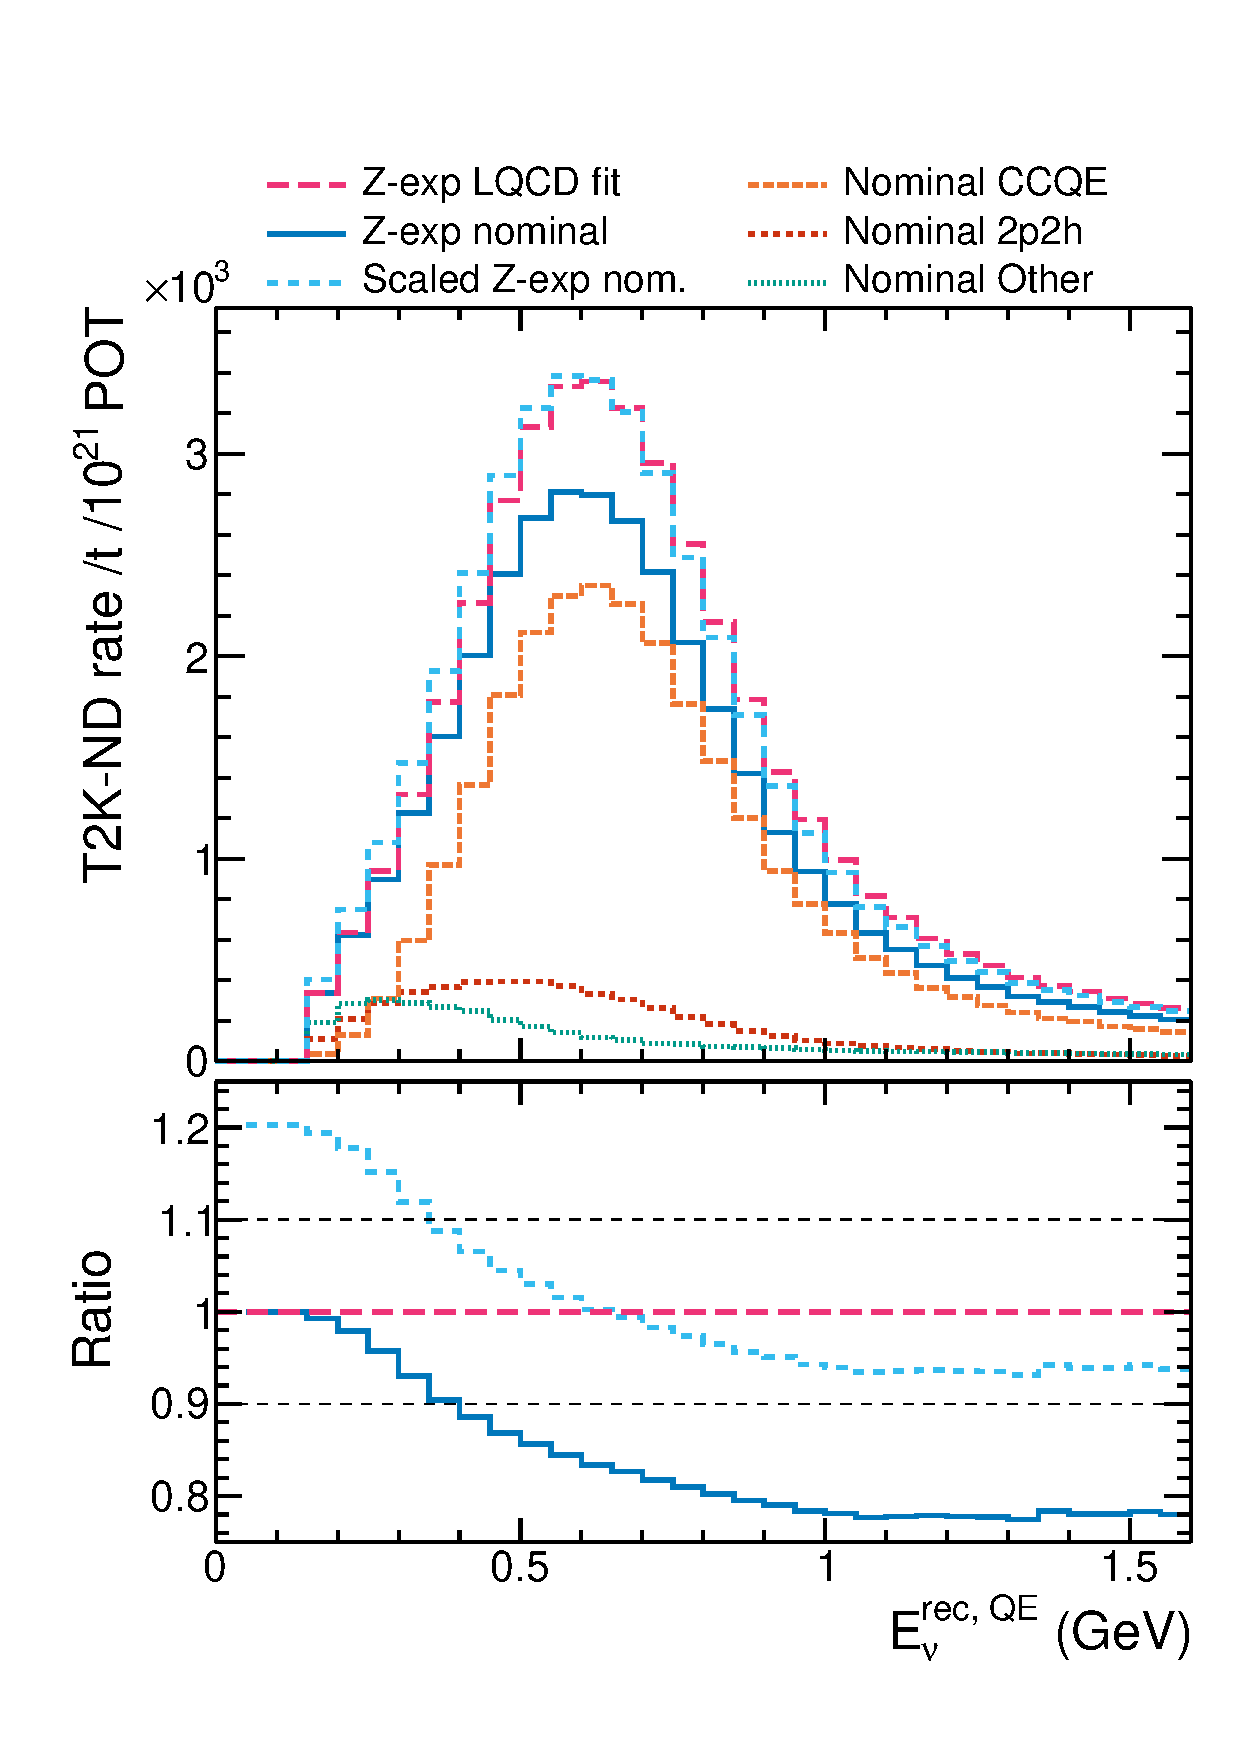
\includegraphics[width=0.3\textwidth]{plots/T2KND_numu_H2O_model_comp.pdf}}\hspace{75pt}
  \subfloat[Far detector] {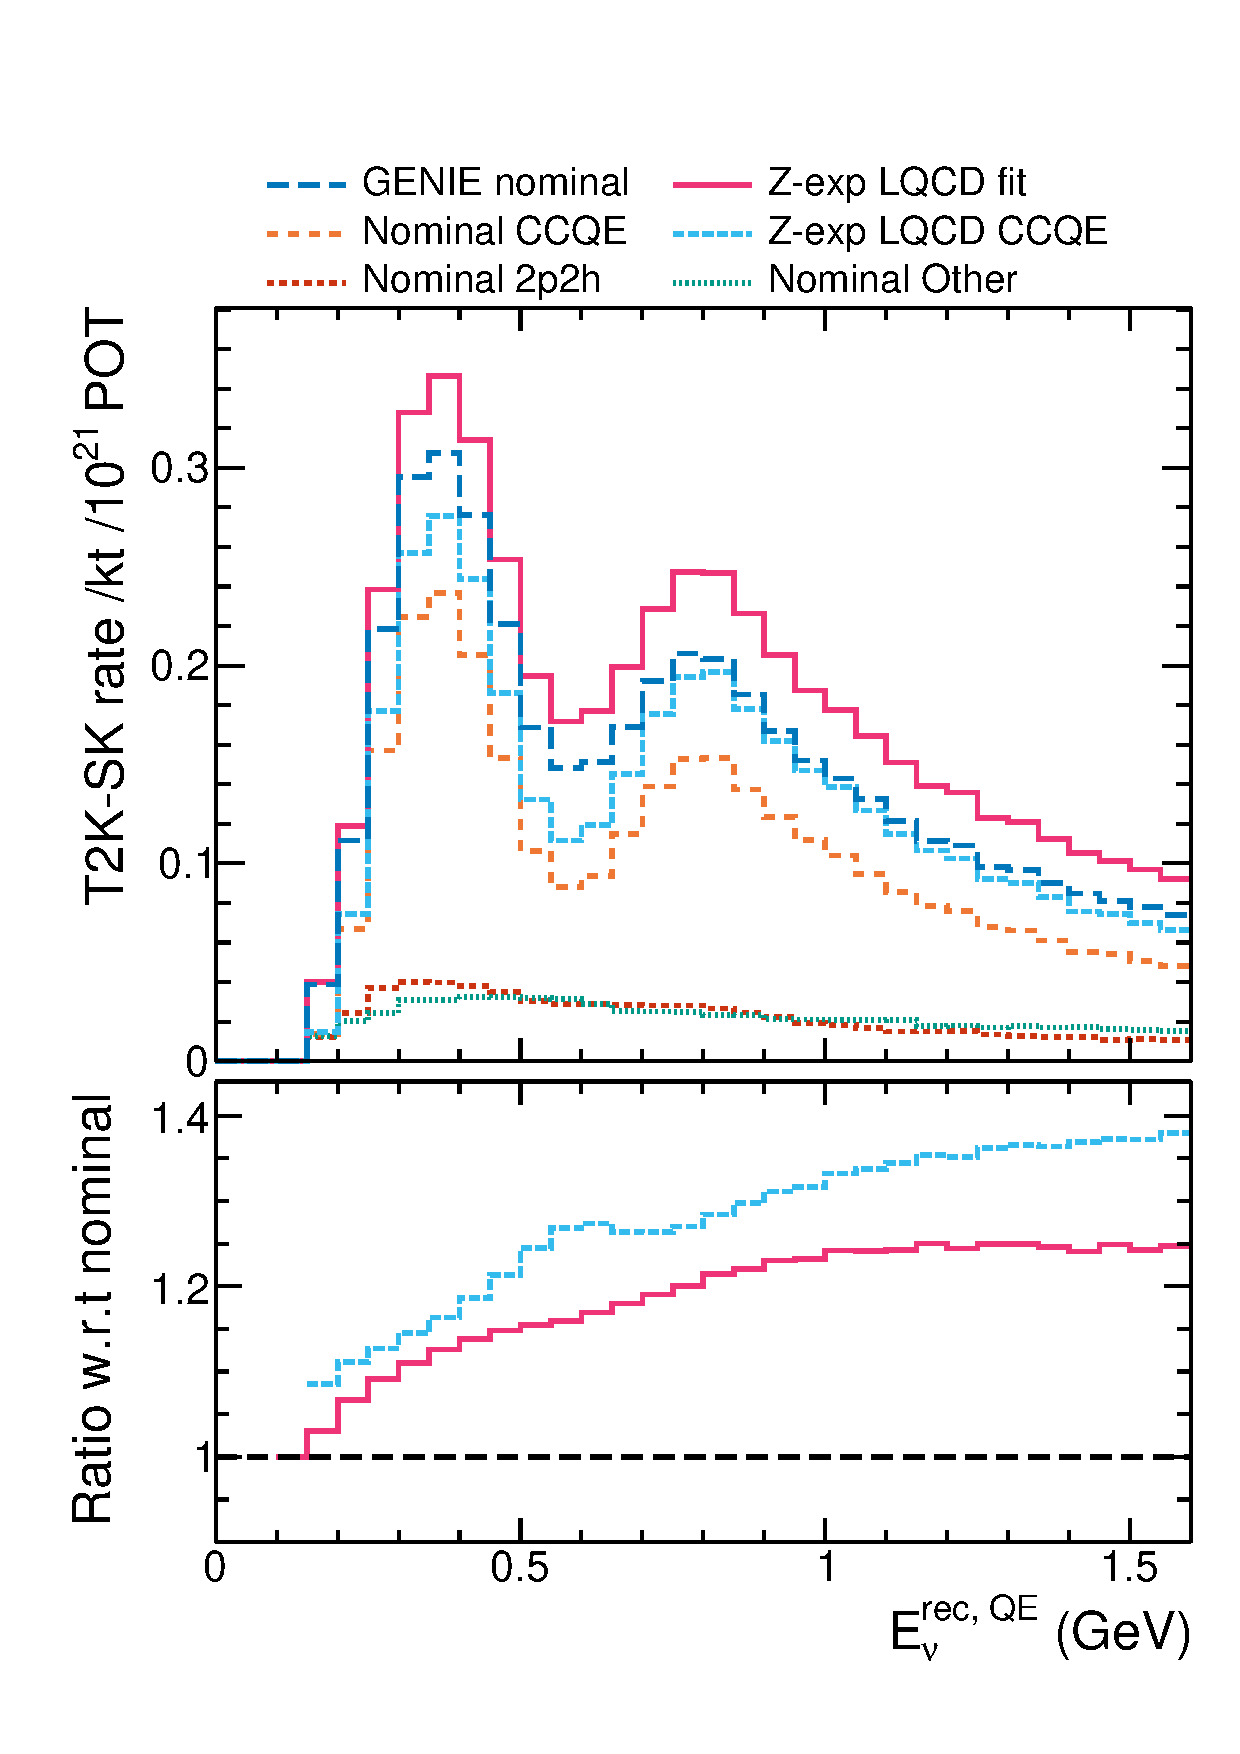
\includegraphics[width=0.3\textwidth]{plots/T2KFD_numu_H2O_osc_model_comp.pdf}}
  \vspace{11pt}
  \caption{The $\nu_{\mu}$--H$_{2}$O CC0$\pi$ event rates per ton (kiloton) per $1\times10^{21}$POT at T2K's near (far) detector site, shown as a function of $E^{\mathrm{rec,\;QE}}_{\nu}$. The GENIE nominal event rate (blue solid line) is produced using the GENIEv3 10a\_02\_11a tune to nucleon data~\addcite{} and the T2K flux~\addcite{}, and the CCQE (orange dashed line), CC-2p2h (red short dashed line) and CC-other (green dotted line) contributions are shown. The oscillated flux is calculated with Ref.~\addcite{}, using the best fit NuFit5.0 oscillation parameters in normal ordering. Additionally, an alternative GENIE model is shown, where the only change is to use the z-expansion model of the axial form factor, with parameters tuned to LQCD results, as described in Section~XYZ. Additionally, the ratio of the nominal to modified GENIE models is shown.}
  \label{fig:t2k_impact}
\end{figure}
Figure~\ref{fig:t2k_impact} shows the $\nu_{\mu}$--H$_{2}$O CC0$\pi$ event rate expected at the T2K near and far detectors for a fixed exposure, with and without modifications to the axial form factor. The nominal GENIEv3 10a\_02\_11a uses a dipole axial form factor with $M_{\mathrm{A}} = 0.941$ GeV$^2$ obtained through a fit to bubble chamber data~\addcite{}. The alternative model shown differs only in the use of the z-expansion model for the axial form factor, with parameters tuned to the LQCD results described in Sectoin~XYZ. The axial form factor change is relevant for all CCQE events, which clearly make up the vast majority of T2K's CC0$\pi$ samples, and it is apparent from Figure~\ref{fig:t2k_impact} that the total event rate has significantly changed as a result, by approximately 20\% in both cases.

It is also clear from the ratios that the change in the total event rate is not purely a normalization change, which is unsurprising as the change only affects CCQE events. However, the ratios are not the same for the near and far detectors, because the relative fractions of the different interaction modes that populate the CC0$\pi$ sample is not the same in the oscillated flux, and they have different $E_{\nu}^{\mathrm{true}}$ --- $E^{\mathrm{rec,\;QE}}_{\nu}$ relationships. This is problematic in a subtle way. In an oscillation analysis, the near detector data serves to constrain the values of all systematic uncertainties that affect the flux, cross section and detector systematic models. If a model is deficient, the systematics will be varied in a way that compensates for that deficiency as far as is possible. This is a valuable way to improve an {\it a priori} model with high-statistics data, but, it introduces the possibility for adding a bias if the deficiency is attributed to the wrong interaction mode. This is very likely to happen if different interaction modes have different relative freedom to change due to larger systematic uncertainties.



\begin{figure}[htbp]
  \centering
  \subfloat[ND]{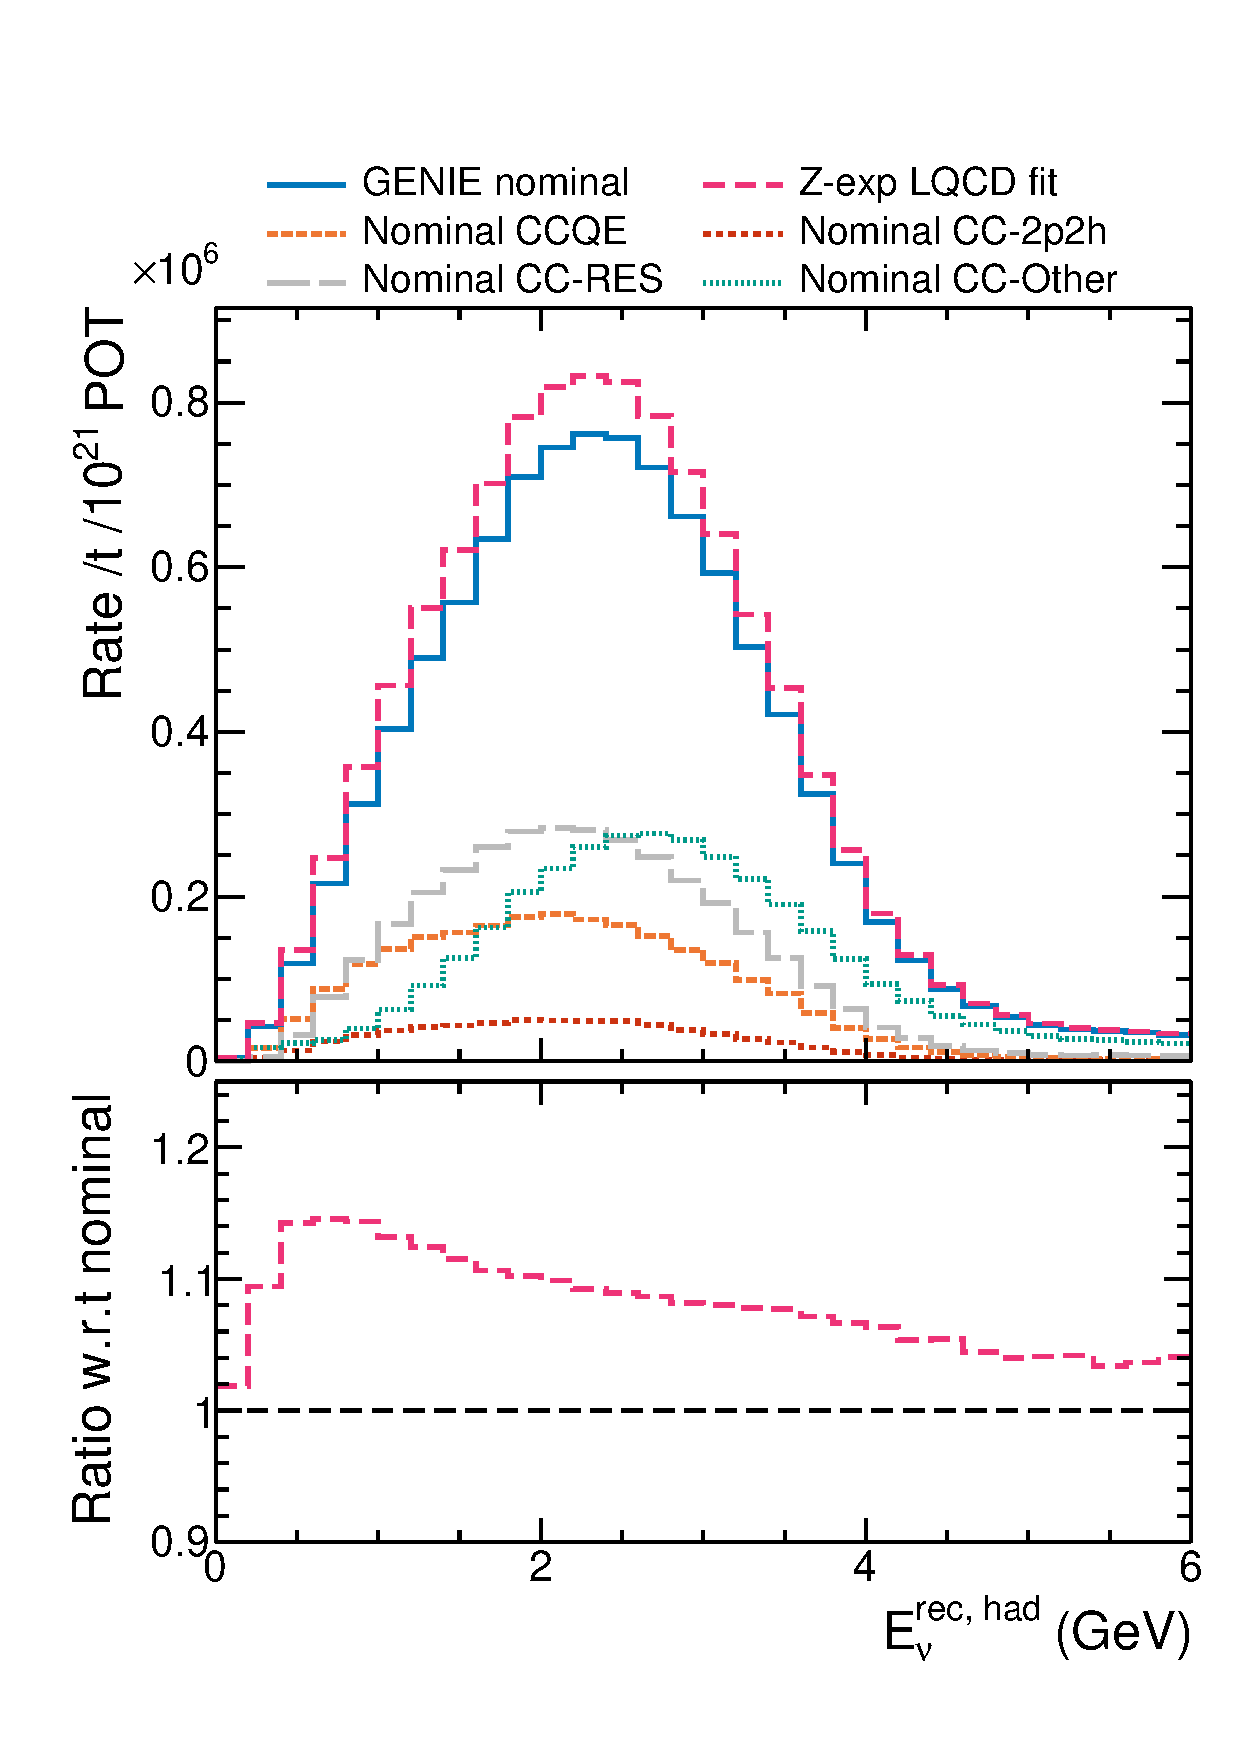
\includegraphics[width=0.3\textwidth]{plots/DUNE_numu_Ar40_breakdown.pdf}}\hspace{75pt}
  \subfloat[FD]{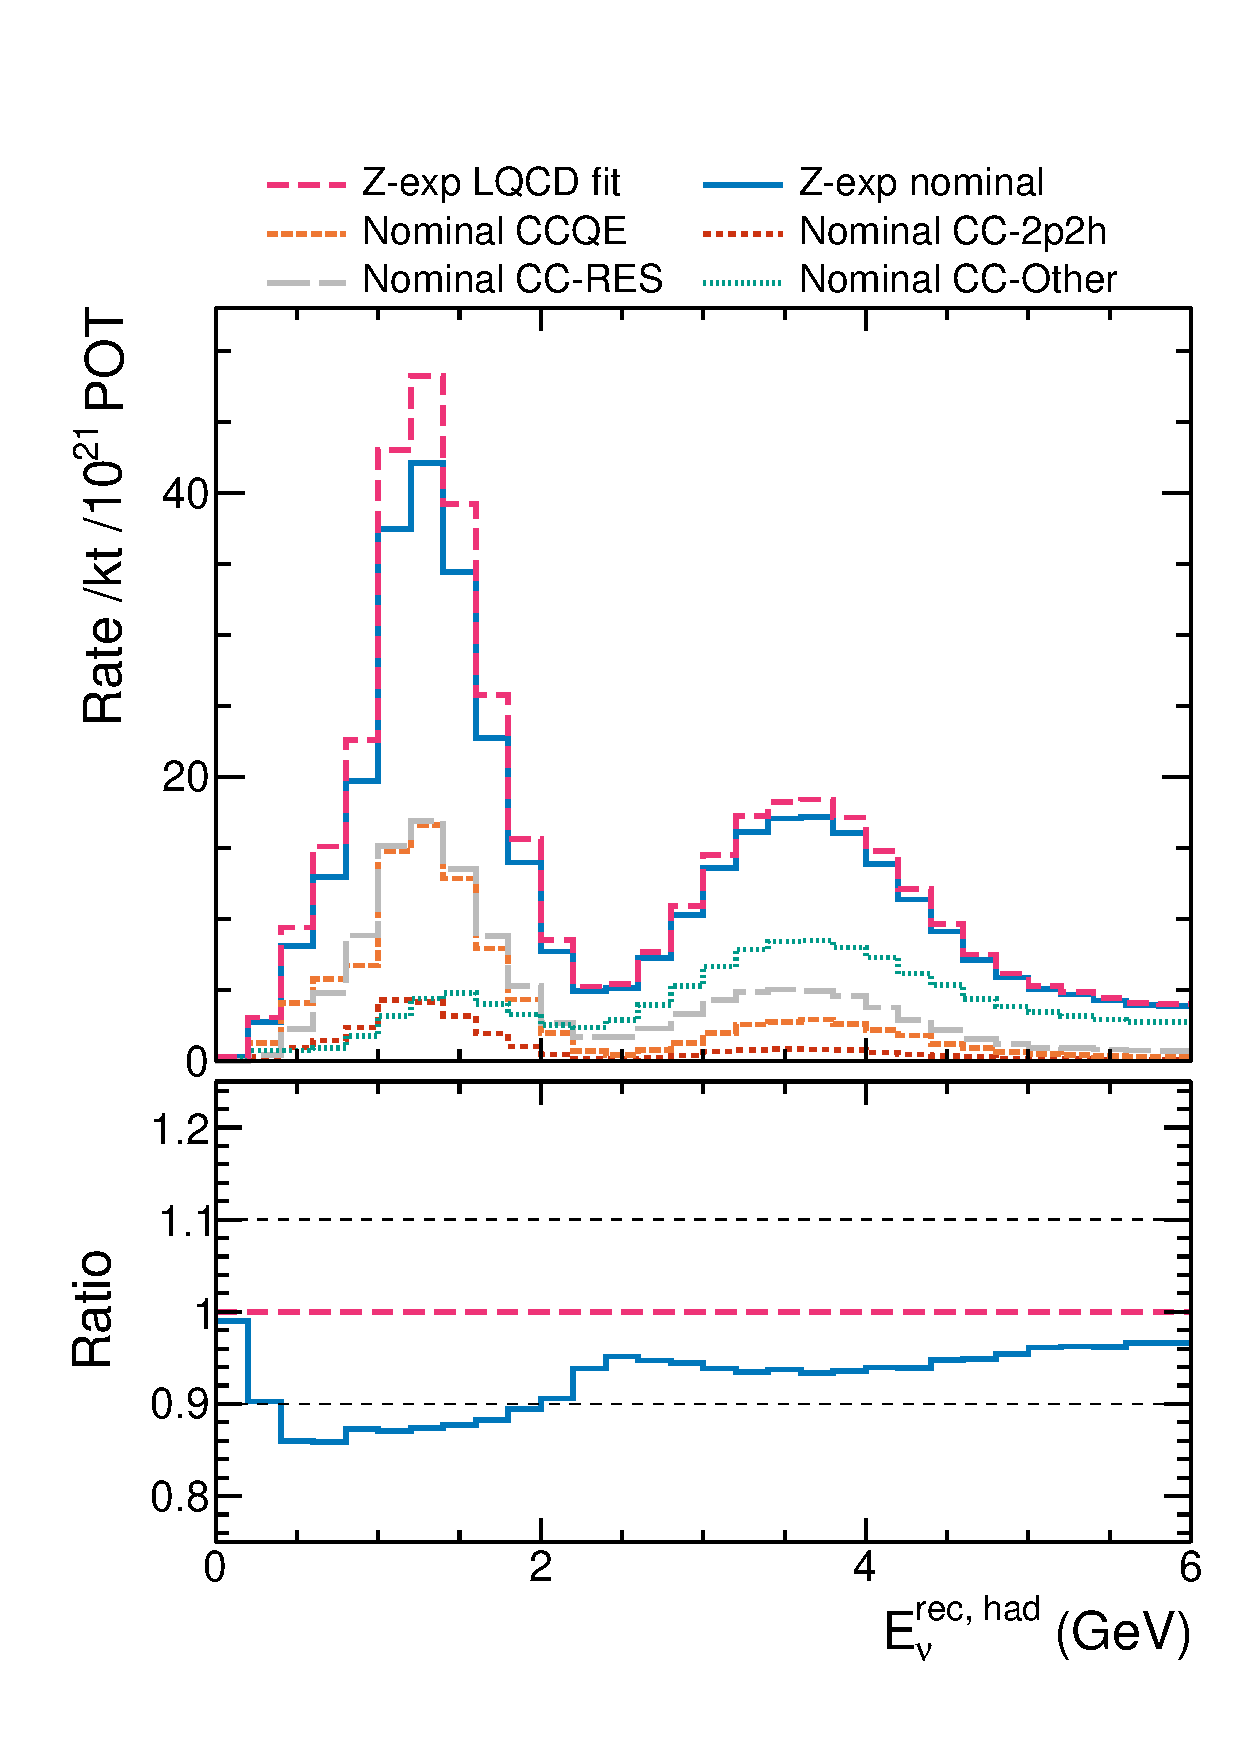
\includegraphics[width=0.3\textwidth]{plots/DUNE_osc_numu_Ar40_breakdown.pdf}}
  \caption{DUNE...}
  \label{fig:dune_impact}
\end{figure}
